\section{Gamification}
\label{sec:gamification}
Gamification is 
\begin{quote}
	the process of game-thinking and game mechanics to engage users and solve problems \cite{Zichermann2011}
\end{quote}
This means using core elements of games to attract users and keep them coming back to a specific task.
Since making the final product engaging is one of our requirements, see \autoref{sec:requirements}, gamification is a natural way of approaching the problem of making this happen.\newline

The video game 'FoldIt', developed at the University of Washington in 2008, employs people in folding proteins.
Folding proteins is a task that the brute-force approach of computers does worse than humans, since humans have natural abilities with regards to spatial reasoning and 3D pattern matching.
In 2011 a team of users managed to decode an virus causing AIDS in monkeys in just 10 days using 'FoldIt'.
This was a task, which had been unsuccessfully attempted by scientists for 15 years.\cite{Huff2011}
Today, the game has almost 500.000 registered users, that use some of their spare time to fold proteins for science for free.\cite{FoldIt2013}\newline

'FoldIt' works, because it employs game mechanics and dynamics, that correlate with some of the primary human desires that will keep people interested and engaged in the activity.
\autoref{fig:bunchball} shows the interaction between human desires, such as status, competition, and reward.
If the game mechanics shown are used, more people would possibly feel entertained while using the product.
This is beneficial to a product that, for example, educates the user. 

\begin{figure}[h]
  \centering
    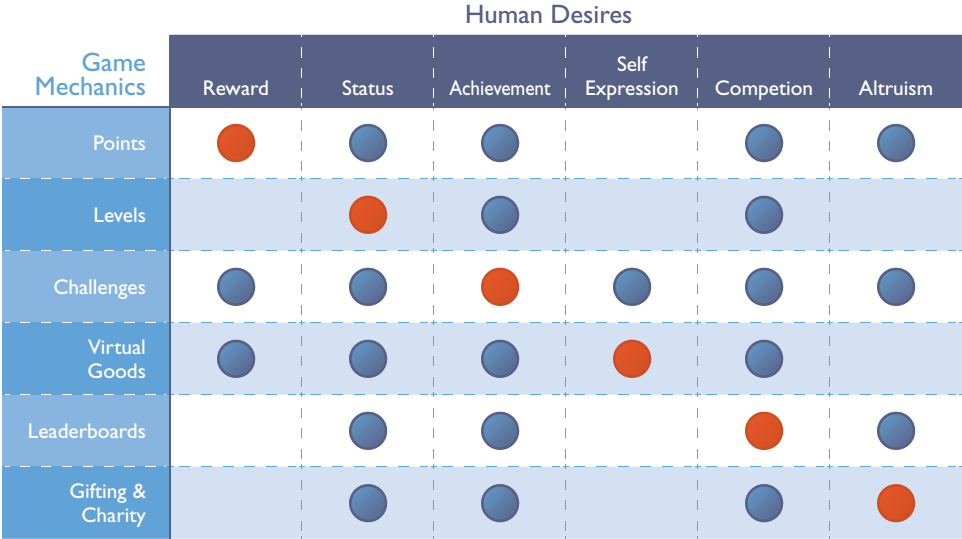
\includegraphics[width=\textwidth]{img/bunchball.png}
  \caption{Interaction between Human desires and Game mechanics}
  \label{fig:bunchball}
\end{figure}

As can be seen in \autoref{fig:bunchball}, the human desires can be fulfilled via various game mechanics.
'FoldIt' utilizes a leaderboard, which allows the users to compete against each other either as groups or soloists.
Allowing both groups and soloists to compete makes the game appealing to both individualists and team players.
If only groups could compete, it might impact the amount of individualists, that would participate.
We see, that appealing to a wider range of character types increase the number of people, that use the game.
This is something, that should be taken into account when developing our game.\newline

In the online application 'FreeRice', developed for the World Food Programme, the user's desire for altruism is fulfilled via donations of rice grains for completed tasks, while general academic skills are honed, such as vocabulary and basic mathematical proficiency. Again, it is possible to join groups, and the game also utilizes a leaderboard, thereby introducing the competition desire.\cite{freerice}\newline

As has been described, the game mechanics illustrated in \autoref{fig:bunchball} will give people an extrinsic motivation (rewards, leaderboards etc.) to keep playing, although the activity might not carry any intrinsic motivation for the user.
This is useful in education, because people tend to easily give up, or simply never really start, when acquiring knowledge and skills that, while useful, may not be their primary field of interest.
Keeping people entertained while learning can ensure that they spend more time on the subject and may also pique their interest in an area, that they might not have explored by themselves.
We see that challenges is the only game mechanic to engage all the human desires, which is why challenges could be introduced earlier than for example levels and leaderboards.